\documentclass[a4paper,10pt]{article}

\usepackage[utf8]{inputenc}
\usepackage{t1enc}
\usepackage[spanish]{babel}
\usepackage[pdftex,usenames,dvipsnames]{color}
\usepackage[pdftex]{graphicx}
\usepackage{amsmath}
\usepackage{amsfonts}
\usepackage{amssymb}
\usepackage[table]{xcolor}
\usepackage[small,bf]{caption}
\usepackage{float}
\usepackage{subfig}
\usepackage{listings}
\usepackage{bm}
\usepackage{times}

\setcounter{secnumdepth}{5}

\begin{document}

\begin{titlepage}
	\thispagestyle{empty}
	\begin{center}
		
\includegraphics[scale=0.7]{./images/itba.jpg}
		\vfill
		\Huge{Autómatas, Teoria de Lenguajes y Compiladores}\\
		\vspace{1cm}
		\huge{Trabajo Práctico Especial 1} \\
		\vspace{0.3cm}
		\huge{Title}
	\end{center}
	\vspace{2cm}
	\large{
		\begin{tabular}{lcr}
			Castiglione, Gonzalo & & 49138 \\
			Susnisky, Darío & & 50592 \\
			Ordano, Esteban & & 50753 \\
			Sturla, Martín & & 50684 \\
			\\ 
		\end{tabular}
	}
	\vfill
	\flushright{\today}
\end{titlepage}

\newpage

%%%%%%%%%%%%%%%%%%%%%%%%%%%%%%%%%%
%%%%%%%%% begin CONTENT %%%%%%%%%%
%%%%%%%%%%%%%%%%%%%%%%%%%%%%%%%%%%

	\thispagestyle{empty}
\tableofcontents

\newpage

\setcounter{page}{1}

\newpage

\section{Resumen}
El trabajo práctico consistia en poder leer tanto un autómata como una gramática y transformarlo en su contraparte
 equivalente. Para esto, era necesario leer e interpretar los archivos de entrada con archivos de \textit{lex}.

\newpage

\section{Consideraciones realizadas}
    No hubo consideraciones externas hechas ya que en caso de errores en los archivos de entradas era nuestro trabajo
     detectarlos. Por otra parte, dentro de la lógica del programa si se valida que la gramática sea coherente 
      (por ejemplo que no hayan caracteres repetidos entre los símbolos terminales y los no terminales) y regular
      (en caso que el archivo de entrada sea una gramática). En caso de que el archivo de entrada sea un autómata
      bastaba con chequear su validez como autómata. \\
Como única consideración, en caso de haber un autómata con estados inalcanzables, en vez de rechazarlo con un mensaje de error, 
se decidió simplemente convertirlo a gramática y luego eliminar los símbolos no terminales inalcanzables y sus producciones asociadas.

\newpage

\section{Descripción del desarrollo}
    Al comienzo, pudimos detectar distintos módulos del trábajo. Estos implicaban tanto leer un autómata o una gramática
     y dejar sus datos de forma accesible en las estructuras correctas. Estos \textit{parsers} eran los encargados
      de validar los datos de entrada.
      
      Luego contabamos con los módulos que manipulaban las estructuras, pasando de autómata a gramática y viceversa.
      También era necesario un algoritmo que transforme cualquier tipo de gramáticas regulares en gramáticas 
       regulares derechas.

      Por último, existían los modulos de \textit{output} que debían contemplar tanto el caso en que se quiera imprimir
       un autómata como una grámatica.
      El siguiente gráfico muestra la la estructura que pensamos inicialmente como nuestro programa.

      \begin{center}
      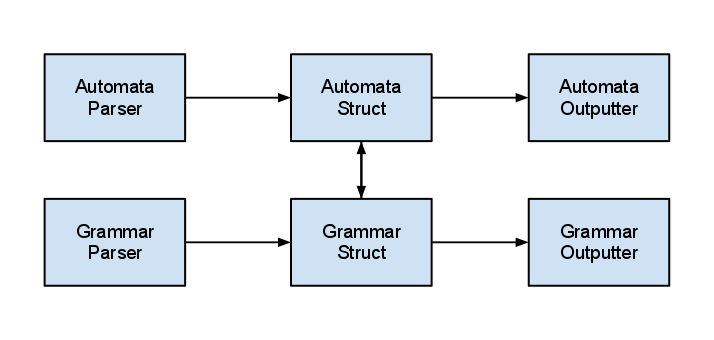
\includegraphics[scale=0.5]{./images/ATL-SegundoDiagrama.png}
      % ATL-SegundoDiagrama.png: 714x340 pixel, 72dpi, 25.19x11.99 cm, bb=0 0 714 340
      \end{center}


      Luego de un segundo análisis comprendimos que no era necesario contar con una estructura que represente
       un autómata, pues era sencillo hacer la conversión entre ambas partes sin contar con esta estructura.
      Así, se formo este segundo diagrama:

      \begin{center}
 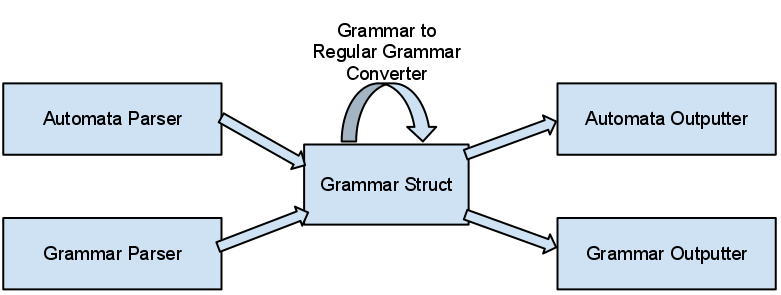
\includegraphics[scale=0.5]{./images/ATL-PrimerDiagrama.png}
 % ATL-PrimerDiagrama.png: 781x295 pixel, 72dpi, 27.55x10.41 cm, bb=0 0 781 295
\end{center}


      Al llegar al final del trabajo, comprendimos que por la manera en que era pedida la muestra de datos,
       era cómodo contar con la estructura que representaba al autómata. Así, nuestra versión final es bastante similar
       a la primera, con la salvedad que dicha estructura solo se usa cuando se lee un autómata de un archivo. Es decir, al leer el autómata 
se crea la estructura de autómata y se la llena con los datos, y luego se convierte a gramática. Esto no es el caso con las gramáticas, ya que 
se contempló que una vez que la gramática está en forma normal derecha, su pasaje a autómata es simple. Por lo tanto, en vez de transformar una estructura 
de tipo gramática a tipo autómata, se decidió que el módulo encargado de imprimir un autómata en un archivo tome una gramática en forma normal derecha 
como entrada y la convierta mientras se imprime ( es decir nunca se pasa por una estructura de tipo autómata de por medio ).

      A continuación se realiza un análisis un poco más profundo en cada uno de los modulos.

      \newpage

      \subsection{Parsers}
            Para realizar la interpretación de los archivos de entrada, primero fue necesario familiarizarse con
            \textit{lex}. Esto era muy importante ya que no podían quedar reglas sin especificar. 
            Luego, fue esencial modelar el \textit{parser} como una maquina de estados. De este modo y teniendo
            todos los estados posibles identificados fue sencillo plasmar código de C que realice lo que cada caso
            requería. 
            Estos procesos fueron llevados a cabo tanto para leer un autómata o una gramática.
      \subsection{Conversión entre estructuras}
            Dados los algoritmos vistos en clase y ciertas pruebas que hicimos fue sencillo ubicar los algoritmos
            para convertir autómatas en gramáticas y viseversa. Nótese que para ambas conversiones, el alfabeto es el mismo (es decir los carácteres 
consumidos en las transiciones del autómata pasan a ser símbolos terminales en la gramática y viceversa).
\subsubsection{Gramática en forma normal derecha a autómata}
Como ya se explicó, la conversión es simple así que se hace mientras se imprime. Se crean mapas para crear equivalencias entre 
símbolos no terminales (un caracter) y un estado (un número). El símbolo distinguido pasa a ser el estado inicial $q_{0}$. Luego para cada producción 
se crea una transición en el autómata con origen en la parte derecha de la producción y destino en el símbolo no terminal de la parte derecha, consumiendo 
el símbolo terminal de la parte derecha. Si la parte derecha de la producción no tiene símbolo no terminal, entonces el destino es un estado final que se 
crea. 
\subsubsection{ Autómata a gramática }
           Para cada estado del autómata, se crea un símbolo no terminal, nuevamente usando mapas de entero a caracter. Luego para cada transición del 
autómata se crea una producción. La parte izquierda de la producción es el símbolo no terminal equivalente al estado origen. La parte derecha de 
la producción es el símbolo terminal equivalente al estado destino (podría en particular ser el mismo). Si la transición consume un caracter, 
se agrega dicho caracter al comienzo de la parte derecha de la producción. Luego, para cada estado final se agrega una producción cuya parte izquierda 
es el símbolo no terminal asociado y cuya parte derecha es simplemente el símbolo $\lambda$. Finalmente el símbolo no terminal asociado al estado inicial 
del autómata pasa a ser el símbolo distinguido.
 
      \subsection{Conversion de gramática a gramática alineada a derecha}
            El algoritmo se basa  en la inversión de todas las producciones de tipo $A->Bc$  a  $B->cA$. Primero se crea un nuevo símbolo terminal, $M$.
Toda producción que no genere de su lado derecho un símbolo no terminal generará lo mismo de antes con $M$ concatenado (en particular si la producción era 
a $\lambda$ se generará una unitaria a $M$). Luego, se invierten todas las producciones como se ha explicado previamente. Tras hacer esto, $M$ pasa a ser el 
nuevo símbolo distinguido. Con esta nueva gramática, se eliminan todos los símbolos inalcanzables y no productivos (utilizando un $BFS$). Por último se 
eliminan las producciones unitarias. Esto se logra recorriendo todas las producciones mientras haya unitarias, y para cada una que lo sea, se reemplaza 
el no terminal a la derecha de dicha producción por todas las posibles partes derechas de sus producciones. 
      \subsection{Output}
            El \textit{output} no presentó una complicación mayor ya que al contar con los formatos de salida 
            requeridos y al tener los datos ordenados en estructuras correctas, el proceso fue casi intuitivo.
            Por otra parte hubo que tener cuidado con el uso de \textit{graphbiz}, pero acompañados de ciertos
            conocimientos previos esto tampoco presento una grán complicación.

\newpage

\section{Dificultades encontradas}
    Más alla de los cambios que hubo que ir haciendo en el diseño de la aplicación y algún que otro \textit{bug} 
    , podemos decir que no nos topamos con dificultades muy grandes. Igualmente, es interesante notar hubo que 
    familiarizarse con la sintaxis de \textit{lex} y que el algoritmo para transformar una gramática en una 
    gramática alineada a dereche no fue sencillo de implementar.
\newpage

\section{Futuras Extensiones}
    Durante el desarrollo surgieron ideas para futuras extensiones al trabajo, enumeradas a continuación:
\subsection{ Autómatas mínimos y determinísticos }
Al leer un archivo de gramática y convertirlo en un autómata equivalente, se podrían implementar algoritmos para minimizar y hacer
determinístico a dicho autómata. Asimismo, al leer un archivo de autómata, se podría indicar por salida estándar si dicho autómata es 
determinístico y mínimo. Para implementar esta extensión, se deberían implementar los algoritmos vistos en las clases teóricas para 
primero convertir el autómata en determinístico y luego aplicar el algoritmo de minimización.
\subsection{Detección de gramáticas regulares}
El programa acepta solo producciones en las formas:
$A->aA | Aa | a | A | \lambda$
Esto garantiza que la gramática de entrada es regular. Si hay una producción que no respeta estas reglas, se descarta porque no es regular. Esto 
puede no ser cierto, dado que una gramática podría tener varios símbolos terminales a la derecha de una producción y generar un lenguaje regular. 
Podríá implementarse un algoritmo que detecte si la gramática es regular, y si lo es, independiente de su forma, intente generar el autómata 
equivalente. El problema es que verificar que el lenguaje generado por una gramática es regular no es una tarea  trivial, y la complejidad de los algoritmos 
para hacerlo podría ser muy alta. Una alternativa más fácil de implementar sería intentar hacer reemplazos en las producciones para intentar llevar todas 
las producciones a forma normal. El problema con este método es que a pesar que todo lenguaje regular tiene al menos una gramática en forma normal 
asociada, intentar llevarla a forma normal puede resultar muy tedioso. Véase el siguiente ejemplo de producción:
$ A->aaabbababababaaaaaA | bbbbaaaabbbbb $
Claramente una gramática con esta única producción es regular, pero pasar dicha producción a forma normal involucaría la creación de muchos símbolos 
no terminales y producciones adicionales.
\end{document}

